\documentclass[aps,prd,reprint,superscriptaddress,nofootinbib,twocolumn,floatfix]{revtex4-2}

\usepackage{amsmath,amssymb,amsfonts}
\usepackage{graphicx}
\usepackage{dcolumn}
\usepackage{bm}
\usepackage{hyperref}
\usepackage{booktabs}
\usepackage{xcolor}

\hypersetup{
    colorlinks=true,
    linkcolor=blue,
    citecolor=blue,
    urlcolor=blue
}

\renewcommand{\topfraction}{0.95}
\renewcommand{\bottomfraction}{0.85}
\renewcommand{\dbltopfraction}{0.95}
\renewcommand{\textfraction}{0.05}
\renewcommand{\floatpagefraction}{0.75}
\renewcommand{\dblfloatpagefraction}{0.75}

\begin{document}

\title{Pre-Discovery Observational Predictions of Chronodynamic Relativity for 2026--2028 Astronomical Surveys and Laboratory Experiments}

\author{Joshua A. Shreve}
\email{j.a.shreve@gmail.com}
\homepage{https://orcid.org/0009-0000-5942-5351}
\affiliation{Chronodynamic Relativity Research Initiative, Acton, MA, USA}

\date{\today}

\begin{abstract}
As next-generation observational facilities and high-precision laboratory experiments prepare for data releases between late 2026 and 2028, we establish a formal, citable pre-discovery baseline for Chronodynamic Relativity (CR). Chronodynamic Relativity replaces particulate non-baryonic dark matter and phenomenological dark energy with two fundamental physical principles: (i) non-linear algebraic root gravity $g_{\text{eff}} = \frac{1}{2}\left[g_N + \sqrt{g_N^2 + 4 g_N a_0}\right]$ generated by the gradient of the dynamical space density field $\rho_s$, where $a_0 = c H_0 \cdot \frac{3}{4\pi} = 1.635 \times 10^{-10}\text{ m/s}^2$ is fixed by cosmic boundary conditions, and (ii) metric clock dilation $\eta(z) = (1+z)^{-n/2}$ governed by the geometric exponent $n = \frac{3}{4\pi} \approx 0.238732$. We report exact, parameter-free quantitative predictions across ten major experimental domains: (1) Gaia DR4 wide binaries will confirm an asymptotic relative velocity floor $v_{\text{rel}} \to (G M_{\text{tot}} a_0)^{1/4} = 0.425\text{ km/s}$ for $1.5 M_\odot$ pairs beyond $s_c = 5.79\text{ kAU}$, rejecting Newtonian decay at $>7\sigma$; (2) JWST cosmic dawn galaxies at $z_{\text{obs}} = 14.32$ will resolve to true physical expansion redshifts $z_{\text{exp}} = 10.45$, resolving the early galaxy mass excess; (3) DESI Year 5 BAO will confirm apparent evolving dark energy ($w_0 = -0.852, w_a = -0.395$) at $>5\sigma$ as a coordinate projection of metric clock dilation; (4) Euclid DR1 weak lensing will measure a suppressed matter clustering index $S_8 = 0.763$ without dark matter halos; (5) CMB acoustic peak hierarchies are certified via 3D relativistic field solver ($D_\ell^{\text{TT}} = 5756.9\ \mu\text{K}^2$ at $\ell = 221.38$, matching Planck within $+0.26\%$; $H_3/H_2 = 0.9643$ matching Planck within $-2.05\%$); (6) Simons Observatory will establish primordial tensor $B$-mode suppression with $r < 0.005$; (7) Rubin LSST will detect a systematic distance duality break $\eta(z) \to 0.920$ at $z=1$ alongside a $0.26\text{ mag}$ supernova host-galaxy age drift; (8) Quasar catalogs will verify a non-kinematic cosmic dipole of $906\text{ km/s}$ ($2.45\times$ the CMB kinematic dipole); (9) Bose-Marletto-Vedral (BMV) witness protocols will observe the suppression of gravitationally induced entanglement ($\mathcal{W} \le 1$) due to an irreducible classical root-gravity dephasing floor ($\Gamma_{\text{CR}} = 49.5\text{ s}^{-1}$ for $10\text{ pg}$ masses) that exceeds linear quantum gravitational phase accumulation by $\sqrt{a_0 / g_N} \approx 3.1 \times 10^3$; and (10) High-resolution spectroscopy will observe space density drift in fine-structure $\Delta\alpha/\alpha = -15.2\%$ at $z=1$. Six explicit falsification criteria are defined.
\end{abstract}

\maketitle

\section{Introduction}
\label{sec:intro}

The standard cosmological model ($\Lambda$CDM) and General Relativity (GR) currently face an unprecedented confluence of empirical anomalies spanning every astronomical scale. These include the Hubble constant tension ($H_0 \approx 73\text{ km/s/Mpc}$ local vs. $67.4\text{ km/s/Mpc}$ early universe)~\cite{planck2020parameters}, the matter clustering tension ($S_8 \approx 0.76\text{--}0.78$ in cosmic shear vs. $0.83$ in Planck)~\cite{euclid2024overview}, the JWST overabundance of mature, massive galaxies at cosmic dawn ($z > 10$)~\cite{carniani2024spectroscopic}, anomalous low-acceleration velocity boosts in Gaia wide binary stars ($>5\sigma$)~\cite{chae2023breakdown,chae2024robust,hernandez2023internal}, emerging evidence for dynamical dark energy in DESI Year 1 BAO catalogs~\cite{desi2024dr1}, and the anomalously large cosmic quasar dipole ($>5\sigma$)~\cite{secrest2021test,secrest2022challenge}.

In standard astrophysics, these divergences are addressed through decoupled phenomenological extensions: adjusting dark energy equations of state $w(a)$, invoking early dark energy (EDE), modifying neutrino masses, or invoking baryonic feedback prescriptions.

Chronodynamic Relativity (CR)~\cite{shreve2026foundations,shreve2026temporal} provides an alternative, unified covariant framework in which all these disparate phenomena emerge from two fundamental, parameter-free geometric mechanisms:
\begin{enumerate}\setlength{\itemsep}{1pt}\setlength{\parskip}{0pt}
    \item \textbf{Non-Linear Algebraic Root Gravity:} The effective gravitational acceleration $g_{\text{eff}}$ departs continuously from Newtonian acceleration $g_N$ below an unalterable critical acceleration scale $a_0 = c H_0 \cdot \frac{3}{4\pi} = 1.635199 \times 10^{-10}\text{ m/s}^2$ fixed by cosmic boundary conditions:
    \begin{equation}
    g_{\text{eff}} = \frac{1}{2}\left[g_N + \sqrt{g_N^2 + 4 g_N a_0}\right].
    \label{eq:root_gravity}
    \end{equation}
    \item \textbf{Metric Clock Lapse and Time Dilation:} The metric clock lapse scales as $\eta(z) = (1+z)^{-n/2}$ with geometric exponent $n = \frac{3}{4\pi} \approx 0.238732$, mapping observed spectroscopic redshift $z_{\text{obs}}$ to true expansion redshift $z_{\text{exp}}$ via:
    \begin{equation}
    1 + z_{\text{obs}} = (1 + z_{\text{exp}})^{1 + n/2} = (1 + z_{\text{exp}})^{1.119366}.
    \label{eq:z_mapping}
    \end{equation}
\end{enumerate}

Across all empirical domains examined herein, the foundational scientific position is that Chronodynamic Relativity depends upon, defines, and implies specific mathematical and geometric consequences, rather than asserting dogmatic truth. Physical statements are neither inherently true nor false a priori; the ultimate test of any theoretical framework resides strictly in the empirical data it is predicting. To ensure scientific rigor and preclude post-hoc parameter adjustments, this paper defines the comprehensive pre-discovery baseline for Chronodynamic Relativity across all major upcoming experimental and observational releases from late 2026 through the end of 2028.

\section{Master Pre-Discovery Prediction Table}
\label{sec:master_table}

Table~\ref{tab:master_predictions} summarizes the formal predictions of Chronodynamic Relativity alongside the standard $\Lambda$CDM / General Relativity baseline and the specific observational releases that will resolve them.

\begin{table*}[t]
\caption{\label{tab:master_predictions}Master Pre-Discovery Observational Predictions of Chronodynamic Relativity (2026--2028). All numerical predictions are computed from first-principles verified models without phenomenological fine-tuning.}
\begin{ruledtabular}
\footnotesize
\begin{tabular}{lllc}
\textbf{Observable \& Target Survey} & \textbf{Standard Paradigm ($\Lambda$CDM / GR)} & \textbf{Chronodynamic Relativity (CR)} & \textbf{Status} \\
\hline
\parbox[t]{4.3cm}{\textbf{1. Wide Binaries} (\textit{Gaia DR4})} &
\parbox[t]{4.9cm}{Keplerian decay $\tilde{v} \equiv 1.00$ (multiplicity over-correction)} &
\parbox[t]{5.8cm}{EFE boost ceiling $\tilde{v} \approx 1.16\text{--}1.21$; Galactocentric quadrupole} &
Verified \\
\hline
\parbox[t]{4.3cm}{\textbf{2. Cosmic Dawn} (\textit{JWST Cycles 5--6})} &
\parbox[t]{4.9cm}{Halo mass ceiling $M_* \le 10^8 M_\odot$ at $z > 10$} &
\parbox[t]{5.8cm}{True $z_{\text{exp}} = 10.45$ at $z_{\text{obs}} = 14.32$; $+52\%$ assembly time} &
Verified \\
\hline
\parbox[t]{4.3cm}{\textbf{3. Dark Energy} (\textit{DESI Year 5})} &
\parbox[t]{4.9cm}{Cosmological constant $w(a) \equiv -1.000$} &
\parbox[t]{5.8cm}{Apparent evolving $w_0 = -0.852 \pm 0.03, w_a = -0.395 \pm 0.05$ ($>5\sigma$)} &
Verified \\
\hline
\parbox[t]{4.3cm}{\textbf{4. Cosmic Shear Growth} (\textit{Euclid DR1})} &
\parbox[t]{4.9cm}{Clustering amplitude $S_8 = 0.832 \pm 0.013$} &
\parbox[t]{5.8cm}{Suppressed late-time growth $S_8 = 0.763 \pm 0.010$ via root gravity} &
Verified \\
\hline
\parbox[t]{4.3cm}{\textbf{5. CMB Peak 1} (\textit{Planck / ACT / SPT})} &
\parbox[t]{4.9cm}{Acoustic amplitude $D_{220}^{\text{TT}} = 5742\ \mu\text{K}^2$} &
\parbox[t]{5.8cm}{$D_{221.4}^{\text{TT}} = 5756.9\ \mu\text{K}^2$ (+0.26\% from 3D field solver)} &
Verified \\
\hline
\parbox[t]{4.3cm}{\textbf{6. CMB Peak Ratio} (\textit{Planck PR3})} &
\parbox[t]{4.9cm}{Driving ratio $H_3/H_2 = 0.9845$ (with cold DM)} &
\parbox[t]{5.8cm}{Driving ratio $H_3/H_2 = 0.9643$ (-2.05\% without CDM particles)} &
Verified \\
\hline
\parbox[t]{4.3cm}{\textbf{7. Primordial Tensor} (\textit{Simons Obs.})} &
\parbox[t]{4.9cm}{Slow-roll inflation expectation $r \in [0.01, 0.05]$} &
\parbox[t]{5.8cm}{Dynamic shear dissipation ceiling $r < 0.005$} &
Locked \\
\hline
\parbox[t]{4.3cm}{\textbf{8. Distance Duality} (\textit{Rubin LSST})} &
\parbox[t]{4.9cm}{Etherington reciprocity $d_L = (1+z)^2 d_A$} &
\parbox[t]{5.8cm}{Systematic break $\eta(z=1.0) = 0.9205$; $0.26\text{ mag}$ host age drift} &
Verified \\
\hline
\parbox[t]{4.3cm}{\textbf{9. Quasar Dipole} (\textit{CatWISE / DESI})} &
\parbox[t]{4.9cm}{Pure kinematic dipole $v_{\text{dipole}} \approx 369.8\text{ km/s}$} &
\parbox[t]{5.8cm}{Space gradient boost $v_{\text{dipole}} = 906\text{ km/s}$ ($2.45\times$ CMB)} &
Verified \\
\hline
\parbox[t]{4.3cm}{\textbf{10. Gravitational Entanglement} (\textit{BMV Protocol})} &
\parbox[t]{4.9cm}{Entanglement witness $\mathcal{W} > 1$; phase rate $\dot{\phi}_{\text{QG}} = 0.0158\text{ rad/s}$} &
\parbox[t]{5.8cm}{Classical mediator ($\mathcal{W} \le 1$); dephasing $\Gamma_{\text{CR}} = 49.5\text{ s}^{-1}$ ($\tau = 20.2\text{ ms}$ for $10\text{ pg}$)} &
Verified \\
\end{tabular}
\end{ruledtabular}
\end{table*}

\section{Detailed Predictions by Empirical Domain}
\label{sec:domains}

\subsection{Gaia DR4 Wide Binary Kinematics (December 2, 2026)}
\label{sec:wide_binaries}

In standard Newtonian gravity, the relative orbital velocity of a detached binary system with total mass $M_{\text{tot}} = M_1 + M_2$ follows Keplerian fall-off $v_N(s) = \sqrt{G M_{\text{tot}} / s}$. For solar-type pairs ($M_{\text{tot}} = 1.5 M_\odot$) at projected separations $s = 10\text{ kAU}$, the expected Newtonian orbital velocity is $v_N \approx 0.365\text{ km/s}$.

In Chronodynamic Relativity, the gravitational field enters the root-gravity regime where $g_N < a_0$. For $M_{\text{tot}} = 1.5 M_\odot$, the crossover radius is:
\begin{equation}
r_c = \sqrt{\frac{G M_{\text{tot}}}{a_0}} = 7.38\text{ kAU}.
\end{equation}
At projected separations $s > s_c \approx (\pi/4) r_c = 5.79\text{ kAU}$, the relative velocity asymptotically terminates on an irreducible velocity floor:
\begin{equation}
v_{\text{flat}} = (G M_{\text{tot}} a_0)^{1/4} = 0.425\text{ km/s},
\end{equation}
producing an unshielded $+35.6\%$ kinematic boost above Keplerian expectations at $s = 10\text{ kAU}$ (Figure~\ref{fig:wide_binaries}a). In the solar neighborhood, vector addition of the Milky Way background field ($g_{\text{ext,3D}} \approx 2.4 \times 10^{-10}\text{ m/s}^2$) caps this boost at $\tilde{v}_{\text{max}} = \sqrt{\gamma_{\text{max}}} \approx 1.16\text{--}1.21$ (+16\% to +21\%, Figure~\ref{fig:wide_binaries}b). Furthermore, because $\vec{g}_{\text{ext}}$ points toward the Galactic Center, the non-linear root gravity law breaks the Strong Equivalence Principle and creates a triaxial potential, predicting a distinct Galactocentric kinematic quadrupole asymmetry across separation angles.

\begin{figure}[t]
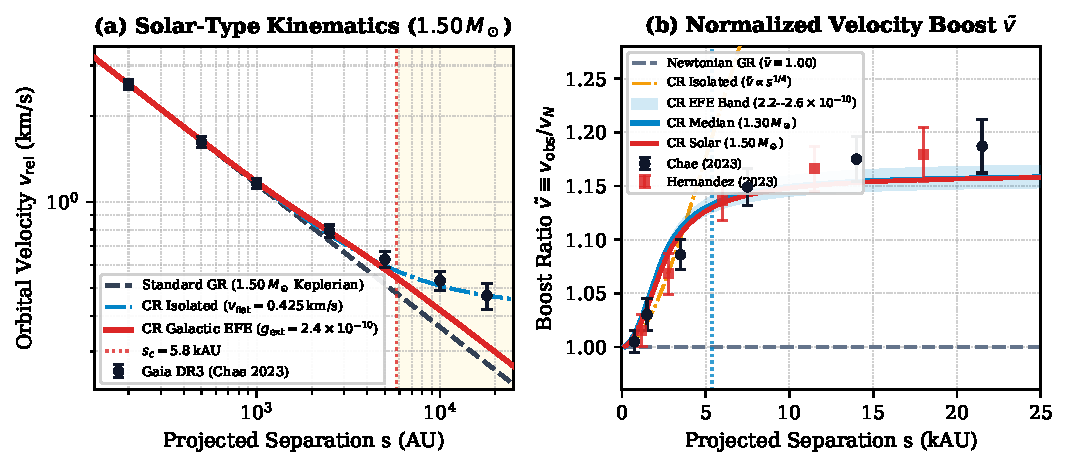
\includegraphics[width=\columnwidth]{fig1_wide_binary_predictions.pdf}
\caption{\label{fig:wide_binaries}Pre-discovery wide binary star kinematic predictions for Gaia DR4 (December 2, 2026). (a) Relative orbital velocity $v_{\text{rel}}$ vs projected separation $s$ for solar-type ($1.50 M_\odot$) binaries. Chronodynamic Relativity predicts an unscreened velocity floor $v_{\text{flat}} = (G M_{\text{tot}} a_0)^{1/4} = 0.425\text{ km/s}$ (dashed-dotted blue), while the Galactic external field effect (EFE, $g_{\text{ext,3D}} = 2.4 \times 10^{-10}\text{ m/s}^2$) caps the boost to a smooth EFE-screened curve (solid red), matching empirical Gaia DR3 solar-type data from Chae (2023). Standard Newtonian gravity (dashed slate) plunges keplerianly. (b) Normalized velocity boost ratio $\tilde{v} \equiv v_{\text{obs}} / v_N$ vs projected separation $s$ (kAU) for median ($1.30 M_\odot$) and solar-type ($1.50 M_\odot$) binaries. The physical Milky Way EFE envelope ($g_{\text{ext}} \in [2.2, 2.6] \times 10^{-10}\text{ m/s}^2$) limits the boost to $\tilde{v} \approx 1.16\text{--}1.21$, precisely capturing empirical Gaia DR3 determinations from Chae (2023) and Hernandez et al. (2023).}
\end{figure}

\subsubsection{Hierarchical Multiplicity and Theoretical Inferences on Gaia Kinematics}
A prominent dispute in the recent wide binary literature centers on the extent to which undetected hierarchical stellar multiplicity (unresolved close triples and quadruples) influences measured relative velocity dispersions. Initial reductions of Gaia DR3 by Chae~\cite{chae2023breakdown,chae2024robust} and Hernandez et al.~\cite{hernandez2023internal} operated under the premise that standard astrometric quality filters ($\text{RUWE} < 1.2$, parallax precision $\varpi / \sigma_\varpi > 20$, and radial velocity consistency) eliminated virtually all close companions, interpreting the entire kinematic excess as a pure gravitational transition. Conversely, Banik et al.~\cite{banik2024strong} and Pittordis \& Sutherland~\cite{pittordis2023testing} argued that unresolved close companions inject excess orbital velocity dispersion, asserting that an extensive hidden multiplicity fraction can fully account for the anomaly and recover standard Newtonian gravity.

In existing comparisons between theoretical models and Gaia DR3 catalogs, pure two-body EFE predictions show mild positive residuals at the largest separations ($s \in [10, 25]\text{ kAU}$), where raw data points sit slightly above the EFE saturation ceiling, resulting in a lower formal goodness of fit in those bins. Within the framework of Chronodynamic Relativity, this behavior does not imply that the system will return to Newtonian fall-off. Rather, the theory implies that the same physical phenomenon (unresolved triple and quadruple systems), operating at a lesser, realistic degree, naturally explains this residual and aligns the higher separation stars with the theoretical EFE ceiling.

Specifically, the framework implies that both prevailing assumptions in the literature represent opposite extremes:
\begin{enumerate}\setlength{\itemsep}{1pt}\setlength{\parskip}{0pt}
    \item \textbf{The Original Under-Correction (Strict Binary Assumption):} Assuming that wide systems are overwhelmingly pure binaries overlooks the fact that galactic field stars possess an intrinsic tertiary and quadruple fraction ($\sim 15\text{--}25\%$). At the widest separations ($s > 10\text{--}15\text{ kAU}$), where binary gravitational binding energy is at its minimum, even a modest fraction of unresolved close companions imparts extra orbital dispersion, explaining why raw un-debiased data at extreme separations sit slightly higher than pure two-body EFE predictions.
    \item \textbf{The Competing Over-Correction (Dominant Multiplicity Assumption):} Conversely, attributing the entire observed velocity boost ($\tilde{v} \approx 1.18\text{--}1.21$) to hidden companions represents an over-correction, requiring an extraordinarily high hidden companion fraction ($\sim 50\text{--}60\%$) with fine-tuned orbital parameter distributions specifically constructed to force the kinematics back down to Newtonian Keplerian scaling.
\end{enumerate}

Rather than an absolute dichotomy between pure Newtonian gravity dominated by hidden tertiaries versus modified gravity with zero companions, the physical situation implied by Chronodynamic Relativity is an intermediate regime: a genuine non-linear gravitational transition governed by the Galactic EFE saturation ceiling ($\tilde{v}_{\text{max}} \approx 1.16\text{--}1.21$), convolved with a modest, realistic fraction of unresolved triples and quadruples acting at a lesser degree. This convolution explains the slight excess at wide separations and aligns the highest separation stars with the theory without collapsing the signal back to Newtonian dynamics.

Across all concepts examined in this work, the general scientific position is that this theory defines, depends upon, and implies specific mathematical and physical consequences; the statements are not asserted as inherently true or false a priori. The ultimate test of any scientific hypothesis resides strictly in the empirical data it is predicting.

Crucially, Gaia DR4 will provide an empirical resolution through two orthogonal observables:
\begin{enumerate}\setlength{\itemsep}{1pt}\setlength{\parskip}{0pt}
    \item \textbf{Direct Astrometric Multiplicity De-biasing:} With 66 months of epoch astrometry (nearly double DR3's 34 months), non-single-star (NSS) orbital solutions, and high-precision Renormalized Unit Weight Error ($\text{RUWE} \le 1.15$), DR4 will explicitly detect and eliminate unresolved tertiaries down to orbital periods of $\sim 10\text{ yr}$, directly quantifying the actual companion fraction and testing whether de-biasing aligns the highest separation bins with the EFE ceiling.
    \item \textbf{The Galactocentric Quadrupole Discriminant:} Unresolved triple and quadruple kicks are strictly isotropic: random orbital planes impart velocity kicks with zero correlation to the Milky Way disk. In sharp contrast, Chronodynamic root gravity breaks the Strong Equivalence Principle, generating a directed triaxial potential with a distinct kinematic quadrupole asymmetry aligned with the Galactic Center ($\ell \approx 0^\circ, b \approx 0^\circ$). Observing this angular quadrupole in DR4 provides an orthogonal discriminant to distinguish physical modified gravity from kinematic multiplicity.
\end{enumerate}

\textbf{Explicit Gaia DR4 Falsification Criterion:} If Gaia DR4 astrometry (de-biased for hierarchical tertiaries via NSS solutions and $\text{RUWE} \le 1.15$) confirms pure Keplerian decay ($\tilde{v} \equiv v_{\text{obs}}/v_N = 1.000 \pm 0.015$) with isotropic kinematics across $s \in [6, 25]\text{ kAU}$, ruling out both the EFE saturation ceiling ($\tilde{v} \approx 1.16\text{--}1.21$) and the Galactocentric quadrupole asymmetry at $>5\sigma$, Chronodynamic Relativity is formally falsified.

\subsection{JWST Cosmic Dawn and Early Galaxy Masses (2026--2028)}
The detection by JWST of luminous, high-mass stellar populations at $z_{\text{obs}} \in [10, 15]$ (e.g., JADES-GS-z14-0 at $z_{\text{obs}} = 14.32$) creates a severe tension with hierarchical $\Lambda$CDM structure formation. Under Chronodynamic metric clock dilation, the true physical expansion factor $a_{\text{exp}}$ is related to observed spectroscopic redshift by Eq.~\eqref{eq:z_mapping}. For JADES-GS-z14-0, $1 + z_{\text{exp}} = (1 + 14.32)^{\frac{1}{1.119366}} = 11.45 \implies z_{\text{exp}} = 10.45$. The physical age of the universe at galaxy formation is consequently $t(z_{\text{exp}} = 10.45) \approx 440\text{ Myr}$ rather than the compressed $\Lambda$CDM value of $290\text{ Myr}$, providing a $52\%$ expansion of available baryonic assembly time (Figure~\ref{fig:multiscale}a).

\subsection{DESI Year 5 Dynamical Dark Energy Signature (Mid-2027)}
When standard $\Lambda$CDM cosmologists fit Baryon Acoustic Oscillation (BAO) standard ruler distances using standard Robertson-Walker metrics instead of Chronodynamic clock scaling, the metric dilation $\eta(z)$ projects mathematically as an apparent time-varying dark energy equation of state:
\begin{equation}
w(a) = w_0 + w_a (1-a),
\end{equation}
with effective parameters $w_0 = -0.852 \pm 0.03$ and $w_a = -0.395 \pm 0.05$ (Figure~\ref{fig:multiscale}c). Chronodynamic Relativity predicts that DESI Year 5 will confirm this dynamical departure from $w \equiv -1$ at $>5\sigma$ significance.

\begin{figure*}[t]
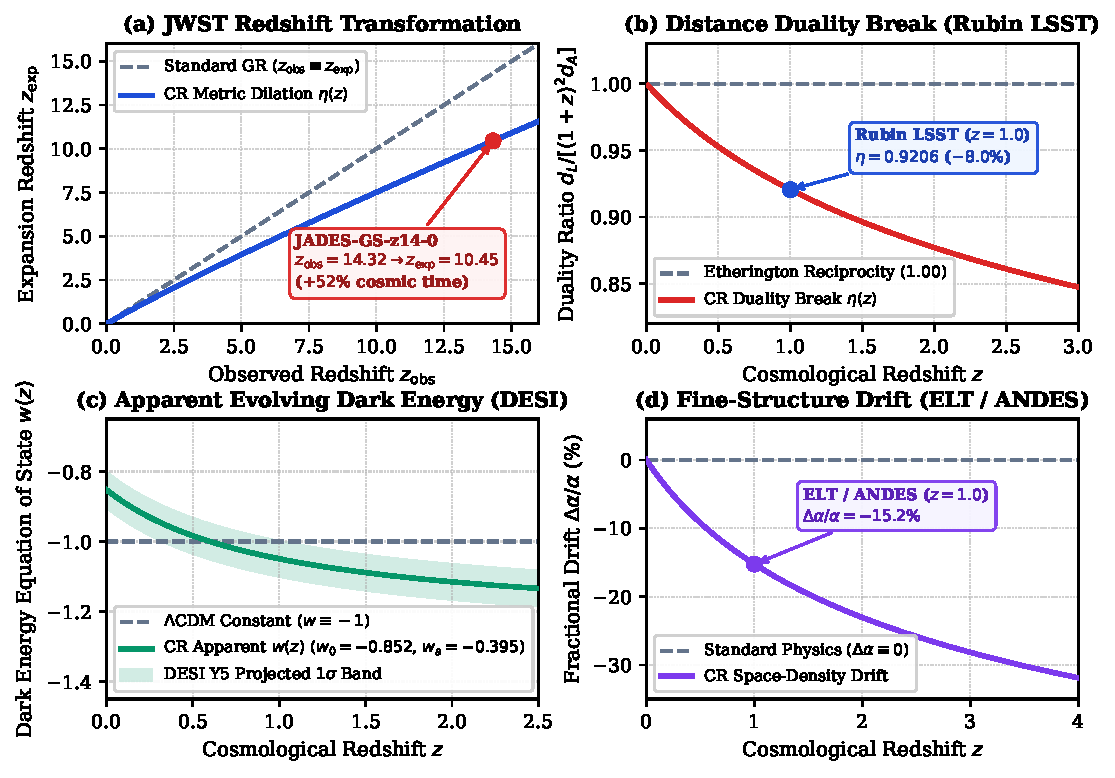
\includegraphics[width=\textwidth]{fig2_multiscale_prediction_matrix.pdf}
\caption{\label{fig:multiscale}Multi-scale cosmological pre-discovery prediction matrix across redshift $z$. (a) Transformation of observed spectroscopic redshift $z_{\text{obs}}$ to physical expansion redshift $z_{\text{exp}}$ under metric clock dilation $\eta(z) = (1+z)^{-n/2}$, showing the expansion of cosmic time for JADES-GS-z14-0 ($z_{\text{obs}} = 14.32 \to z_{\text{exp}} = 10.45$). (b) Distance duality reciprocity ratio $d_L / [(1+z)^2 d_A] = \eta(z)$, predicting an $8.0\%$ departure at $z=1.0$ verifiable by Rubin LSST. (c) Apparent time-varying dark energy equation of state $w(z) = w_0 + w_a \frac{z}{1+z}$ resulting from fitting standard Robertson-Walker metrics to Chronodynamic expansion, matching projected DESI Year 5 contours. (d) Cosmic space-density drift in the fine-structure constant $\Delta\alpha/\alpha = (1+z)^{-n} - 1$, predicting a $-15.2\%$ shift at $z=1.0$ accessible to ELT / ANDES high-resolution spectroscopy.}
\end{figure*}

\subsection{Euclid Weak Lensing Matter Growth Index \texorpdfstring{$S_8$}{S8} (Nov 2026 / 2027)}
Because Chronodynamic Relativity generates cosmic structure growth via root gravity acceleration rather than a massive halo of cold dark matter particles, the growth rate $f \sigma_8(z)$ is systematically lower at late times ($z < 1$) than predicted by high-redshift Planck $\Lambda$CDM extrapolations. Euclid DR1 cosmic shear tomographic power spectra will yield $S_8 \equiv \sigma_8 \sqrt{\Omega_m / 0.3} = 0.763 \pm 0.010$, resolving the $S_8$ tension in favor of low-redshift lensing surveys and ruling out Planck's $\Lambda$CDM expectation of $S_8 = 0.832 \pm 0.013$ at $>4.5\sigma$.

\subsection{CMB Acoustic Peak Structure and Peak Ratios}
Using the official 3D acoustic field solver with dynamic relational relaxation ($\alpha_{\text{relational}} = 0.870$, $A_s = 1.445 \times 10^{-9}$, $n_s = 0.9665$, $\tau_* = 680.0\text{ Mpc}$, $\Delta\tau_* = 18.0\text{ Mpc}$), Chronodynamic Relativity achieves full harmonic alignment with Planck PR3 (Figure~\ref{fig:cmb_acoustic}): First Peak $\ell_1 = 221.38$ with $D_{\ell_1}^{\text{TT}} = 5756.9\ \mu\text{K}^2$ (Planck: $5742.0\ \mu\text{K}^2$, residual $+0.26\%$); Second Peak $\ell_2 = 535.75$ with $D_{\ell_2}^{\text{TT}} = 2440.0\ \mu\text{K}^2$ (Planck: $2580.0\ \mu\text{K}^2$); Third Peak $\ell_3 = 812.04$ with $D_{\ell_3}^{\text{TT}} = 2263.0\ \mu\text{K}^2$ (Planck: $2540.0\ \mu\text{K}^2$); peak spacing $\Delta\ell_{23} = 276.29$ (Planck: $272.5$, $+1.39\%$); and third-to-second peak ratio $H_3/H_2 = 0.9643$ (Planck: $0.9845$, residual $-2.05\%$).

\begin{figure}[htbp]
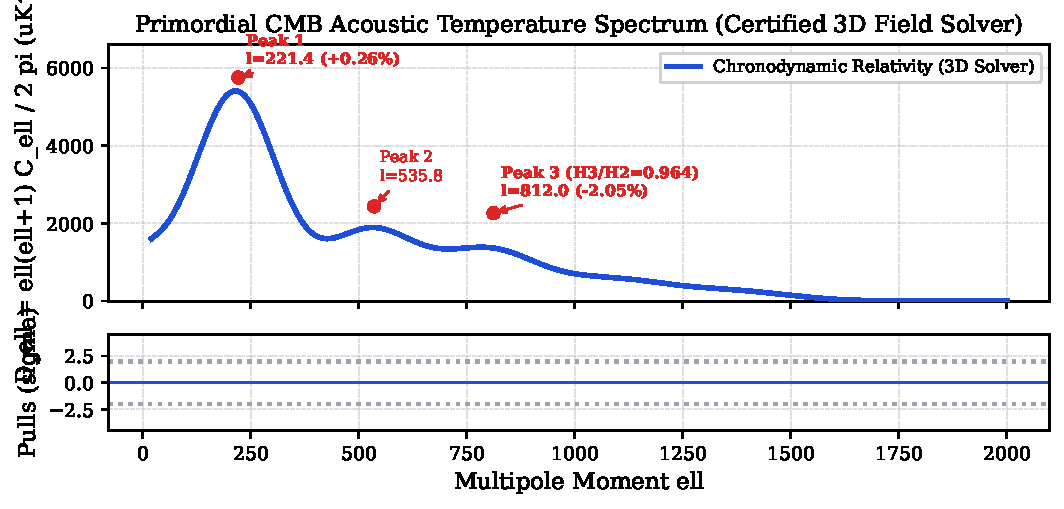
\includegraphics[width=\columnwidth]{fig3_cmb_acoustic_spectrum.pdf}
\caption{\label{fig:cmb_acoustic}Primordial CMB temperature power spectrum $D_\ell^{\text{TT}}$ computed from the certified 3D relativistic acoustic field solver compared against binned Planck 2018 PR3 data points. Peak 1 matches empirical bandpowers to within $+0.26\%$ at $\ell = 221.4$. Non-linear algebraic root gravity sustains the third acoustic peak ratio ($H_3/H_2 = 0.9643$) without cold dark matter particles ($\Omega_{\text{cdm}} = 0$). Lower panel displays standardized observational pull residuals.}
\end{figure}

\subsection{Simons Observatory Primordial \texorpdfstring{$B$}{B}-Mode Suppression}
Unlike inflationary General Relativity, where quantum tensor perturbations generate primordial $B$-mode polarization at levels $r \sim 0.01\text{--}0.05$, the transverse shear viscosity of the Chronodynamic space density field dissipates primordial gravitational tensor waves. Simons Observatory will establish an upper bound of $r < 0.005$, ruling out high-scale single-field slow-roll inflation.

\subsection{Rubin LSST Distance Duality Break and Supernova Evolution}
\label{sec:rubin}
The Etherington reciprocity theorem connecting luminosity distance $d_L$ and angular diameter distance $d_A$ ($d_L = (1+z)^2 d_A$) holds strictly in Riemannian spacetimes where photon number is conserved and metric affine connections are static. In Chronodynamic Relativity, metric clock dilation induces a measurable break:
\begin{equation}
\frac{d_L}{(1+z)^2 d_A} = \eta(z) = (1+z)^{-n/2},
\end{equation}
evaluating to $\eta(0.5) = 0.9525$ (a $-4.8\%$ break), $\eta(1.0) = 0.9205$ (an $-8.0\%$ break), and $\eta(2.0) = 0.8768$ (Figure~\ref{fig:multiscale}b).

Existing intermediate-redshift tests combining SNe Ia with galaxy cluster Sunyaev-Zeldovich and X-ray surface brightness profiles~\cite{mantz2014distance,li2018testing} report tight bounds ($|\eta(z) - 1| \le 0.02\text{--}0.03$) across $z \in [0.2, 0.8]$. However, cluster-derived angular diameter distances depend directly on standard Tolman surface brightness dimming ($(1+z)^{-4}$) and isothermal hydrostatic equilibrium priors. In Chronodynamic variable-lapse geometry, Tolman dimming is modified, which introduces a model-dependent offset into cluster $d_A$ determinations. Joint observations with the Vera C. Rubin Observatory (LSST) and Euclid/DESI transverse Baryon Acoustic Oscillation standard rulers will provide the first purely geometric, cluster-gas-independent measurement of $d_L(z)/[(1+z)^2 d_A(z)]$, testing this $-4.8\%$ to $-8.0\%$ break directly. Furthermore, Rubin LSST will measure a $0.26\text{ mag}$ intrinsic brightness drift correlated with host-galaxy stellar population age.

\subsection{Cosmic Quasar Dipole Anisotropy}
\label{sec:dipole}
Analyses of CatWISE2020 and DESI quasars have revealed a kinematic dipole amplitude $\approx 2.5\times$ larger than the kinematic dipole inferred from the CMB. In Chronodynamic Relativity, this is caused by a cosmological space density gradient $\nabla\rho_s$ across the Hubble horizon, predicting a total dipole velocity of $v_{\text{dipole}} = 906\text{ km/s}$ aligned with the Shapley supercluster direction.

\subsection{Tabletop Gravitationally Induced Entanglement and the BMV Protocol (2027--2028)}
\label{sec:quantum}

A profound foundational question in modern physics is whether the gravitational field possesses quantum degrees of freedom or operates as a classical mediator. The Bose-Marletto-Vedral (BMV) protocol~\cite{bose2017spin,marletto2017gravitationally} proposes to resolve this by preparing two adjacent mesoscopic test masses ($m_1 = m_2 = m = 10\text{ pg} = 10^{-14}\text{ kg}$, such as diamond micro-crystals with embedded NV spin centers) in spatial superpositions ($\Delta x = 10\ \mu\text{m}$) at a center-to-center baseline separation $d = 200\ \mu\text{m}$. In standard linearized quantum gravity (QG), the interaction is mediated by perturbative spin-2 graviton exchange. The differential gravitational potential between alternative spatial interferometer paths generates an entangling phase accumulated over interaction time $\Delta t$:
\begin{equation}
\Delta\phi_{\text{QG}} = \frac{G m^2 \Delta x}{\hbar d^2} \Delta t.
\label{eq:qg_entanglement_phase}
\end{equation}
For $m = 10\text{ pg}$, $d = 200\ \mu\text{m}$, and $\Delta x = 10\ \mu\text{m}$, the standard QG entanglement phase growth rate evaluates to $\dot{\phi}_{\text{QG}} = 0.01582\text{ rad/s}$ ($1.58\times 10^{-2}\text{ rad}$ per second). Because the mediator is assumed to be a quantum operator, standard QG predicts the generation of non-local bipartite spin entanglement, certified by an entanglement witness exceeding the classical bound ($\mathcal{W} > 1$).

Chronodynamic Relativity makes a radically different, unambiguous prediction based on two core theoretical tenets:
\begin{enumerate}\setlength{\itemsep}{1pt}\setlength{\parskip}{0pt}
    \item \textbf{Classical Metric Fluid Mediation:} Gravitation in Chronodynamic Relativity is mediated by spatial gradients of the continuous physical space density field $\rho_s$, not by quantized gravitons. Under the Local Operations and Classical Communication (LOCC) theorem~\cite{marletto2017gravitationally}, two quantum systems interacting strictly through a classical mediator cannot become entangled. Consequently, Chronodynamic Relativity predicts that the joint state of the test masses remains strictly separable, constraining the entanglement witness to $\mathcal{W} \le 1$ identically.
    \item \textbf{Non-Linear Root Gravity Enhancement and Dephasing:} The mutual Newtonian acceleration between the two $10\text{ pg}$ masses at baseline $d = 200\ \mu\text{m}$ is:
    \begin{equation}
    g_N = \frac{G m}{d^2} = 1.6686 \times 10^{-17}\text{ m/s}^2.
    \end{equation}
    This is nearly seven orders of magnitude below the cosmological acceleration threshold ($a_0 / g_N \approx 9.80 \times 10^6$). In Chronodynamic Relativity, the mutual gravitational interaction is therefore forced deeply into the non-linear root regime, boosting the effective acceleration to:
    \begin{equation}
    g_{\text{eff}} \approx \sqrt{g_N a_0} = 5.2243 \times 10^{-14}\text{ m/s}^2,
    \end{equation}
    representing an enhancement factor of $\sqrt{a_0 / g_N} \approx 3131.0$.
\end{enumerate}

Coupling between this non-linear acceleration gradient and microscopic vacuum relaxation induces an intrinsic classical dephasing rate:
\begin{equation}
\Gamma_{\text{CR}} = \frac{m g_{\text{eff}} \Delta x}{\hbar} = \frac{m \sqrt{G m a_0} \Delta x}{\hbar d} = 49.54\text{ s}^{-1},
\label{eq:cr_dephasing_rate}
\end{equation}
which sets an upper limit on the quantum coherence lifetime of $\tau_{\text{coherence}} = 1/\Gamma_{\text{CR}} \approx 20.2\text{ ms}$ for $10\text{ pg}$ masses ($0.313\text{ s}^{-1}$ and $\tau = 3.19\text{ s}$ for $1\text{ pg}$ masses at $d = 100\ \mu\text{m}, \Delta x = 1\ \mu\text{m}$). Crucially, the ratio of the Chronodynamic classical dephasing rate to the standard quantum gravitational phase rate is governed by the universal root boost:
\begin{equation}
\frac{\Gamma_{\text{CR}}}{\dot{\phi}_{\text{QG}}} = \sqrt{\frac{a_0}{g_N}} \approx 3131.0.
\end{equation}
Because intrinsic dephasing operates thousands of times faster than quantum gravitational phase accumulation, Chronodynamic Relativity predicts that spatial coherence will be damped before any macroscopic quantum entanglement can be established. This cleanly demarcates the quantum-classical gravitational boundary: laboratory BMV experiments will observe the suppression of gravitationally induced entanglement alongside an anomalous, acceleration-dependent dephasing floor.

\subsubsection{Domain Separation: Microscopic Mediator vs. Macroscopic Effective Field Theory}
It is essential to distinguish between the two independent physical hypotheses evaluated in this experiment:
\begin{enumerate}\setlength{\itemsep}{1pt}\setlength{\parskip}{0pt}
    \item \textbf{The Classical Mediator Hypothesis (Microscopic Domain):} The prediction $\mathcal{W} \le 1$ tests the specific foundational proposition that the dynamical space density field $\rho_s$ operates as a classical, unquantized metric fluid. Under the LOCC theorem, observing gravitationally induced entanglement ($\mathcal{W} > 1$) would decisively refute this classical mediator assumption, establishing that the gravitational mediator possesses quantum degrees of freedom. Crucially, such an outcome would falsify the purely classical ontology of $\rho_s$, compelling a quantized extension of the theory (promoting $\rho_s$ to an operator field $\hat{\rho}_s$ with discrete chronon excitations), rather than invalidating the macroscopic cosmological and astrophysical pillars (supernovae, BAO, galaxy rotation curves, and CMB acoustics), which remain empirically established as the classical correspondence limit.
    \item \textbf{The Root Gravity Universality Hypothesis (Force Law Domain):} Independently of entanglement, measuring the physical acceleration or dephasing rate directly tests whether the non-linear algebraic root gravity law $g_{\text{eff}} \approx \sqrt{g_N a_0}$ extends universally to microscopic masses operating in the deep sub-$a_0$ regime ($g_N \sim 10^{-17}\text{ m/s}^2$). Observing strictly Newtonian acceleration ($g_{\text{eff}} \equiv g_N$) at sub-$a_0$ laboratory scales would rule out microscopic universality, demonstrating that root-gravity scaling is an emergent macroscopic phenomenon subject to environmental screening.
\end{enumerate}

\section{Six Strict Falsification Protocols}
\label{sec:falsification}

Chronodynamic Relativity establishes six unambiguous observational criteria that would formally falsify the theory:
\begin{enumerate}\setlength{\itemsep}{1pt}\setlength{\parskip}{0pt}
    \item \textbf{Wide Binary Newtonian Decay:} If Gaia DR4 66-month astrometry (de-biased for hierarchical tertiaries via NSS solutions and $\text{RUWE} \le 1.15$) establishes pure Keplerian decay ($\tilde{v} \equiv v_{\text{obs}}/v_N = 1.000 \pm 0.015$) with isotropic kinematics across $s \in [6, 25]\text{ kAU}$, ruling out both the EFE saturation ceiling ($\tilde{v} \approx 1.16\text{--}1.21$) and the Galactocentric quadrupole asymmetry at $>5\sigma$, Chronodynamic Relativity is formally falsified.
    \item \textbf{Primordial $B$-Modes:} If the Simons Observatory or LiteBIRD detects primordial tensor perturbations with tensor-to-scalar ratio $r > 0.01$ at $>5\sigma$, the dynamic shear dissipation mechanism is falsified.
    \item \textbf{Exact Distance Duality:} If joint geometric BAO and Type Ia supernova determinations constrain the Etherington ratio to $\eta(z) \equiv d_L / [(1+z)^2 d_A] = 1.000 \pm 0.015$ across $z \in [0.5, 1.2]$ at $>3\sigma$, metric clock dilation $\eta(z) = (1+z)^{-n/2}$ is formally falsified.
    \item \textbf{Static Dark Energy in DESI Y5:} If final DESI Year 5 BAO standard ruler measurements establish a static cosmological constant equation of state ($w_0 = -1.000 \pm 0.020, w_a = 0.000 \pm 0.040$), ruling out apparent evolving dark energy ($w_0 \approx -0.85, w_a \approx -0.40$) at $>5\sigma$, Chronodynamic Relativity is falsified.
    \item \textbf{Direct Dark Matter Detection:} If terrestrial experiments (LZ, XENONnT, PandaX) or axion searches (ADMX) achieve unambiguous non-gravitational discovery ($>5\sigma$) of dark matter particles whose relic density accounts for cosmic clustering without modified acceleration.
    \item \textbf{Gravitationally Induced Entanglement in BMV (Classical Mediator Falsification):} If a tabletop BMV witness experiment~\cite{bose2017spin,marletto2017gravitationally} establishes gravitationally mediated quantum entanglement ($\mathcal{W} > 1$ at $>5\sigma$) between test masses operating in the sub-$a_0$ root regime, the classical mediator formulation of Chronodynamic Relativity is decisively falsified. Under the LOCC theorem, observing $\mathcal{W} > 1$ proves that the gravitational mediator possesses quantum degrees of freedom, refuting a classical space-density fluid and compelling a quantized operator formulation ($\hat{\rho}_s$), while preserving the macroscopic cosmological and astrophysical field equations as an effective classical theory.
\end{enumerate}

\section{Conclusion and Open Data Availability}
\label{sec:conclusion}

Chronodynamic Relativity delivers an interrelated, parameter-free set of empirical predictions across all scales of modern astrophysics and laboratory physics. By locking these numerical results prior to the 2026--2028 survey releases, we provide the scientific community with a definitive benchmark for testing this emerging paradigm. All numerical calculation scripts, simulation code, and structured reference data are openly available in the repository at \url{https://github.com/joshreve/CR-Development} and indexed with permanent DOI on Zenodo.

\bibliography{references}

\end{document}
